\documentclass[12pt, a4paper]{article}
\usepackage[utf8]{inputenc}
\usepackage[T1]{fontenc}
\usepackage[french]{babel}
\usepackage{geometry}
\usepackage{array}
\usepackage{graphicx}
\usepackage{adjustbox}
\usepackage{xcolor}
\usepackage{tikz}
\usepackage{enumitem}
\usepackage{booktabs}
\usepackage{amsmath}
\usepackage{amssymb}
\usepackage{fancyhdr} % Ajout du package pour les en-têtes

\usetikzlibrary{calc, shapes.geometric}
\geometry{margin=2cm}

% Configuration de l'en-tête
\pagestyle{fancy}
\fancyhf{} % Efface les en-têtes et pieds de page par défaut
\renewcommand{\headrulewidth}{0.4pt}
\renewcommand{\headrule}{\hrule width\headwidth height\headrulewidth}
\fancyhead[C]{\rule{\textwidth}{0.4pt}} % Ligne centrée
\fancyhead[R]{\textit{Investigation numérique}} % Texte à droite
\fancyfoot[C]{\thepage} % Numéro de page centré

% Marges réduites

\definecolor{blue1}{RGB}{0, 51, 102}
\definecolor{blue2}{RGB}{0, 102, 204}
\definecolor{gray1}{RGB}{240, 240, 240}

\begin{document}
	
	\begin{titlepage}
		
		% Bordure autour de la page
		\begin{tikzpicture}[remember picture, overlay]
			\draw[line width=2pt, black] 
			($(current page.north west) + (0.5cm,-0.5cm)$) rectangle 
			($(current page.south east) + (-0.5cm,0.5cm)$);
		\end{tikzpicture}
		
		\centering
		
		% SOLUTION FONCTIONNELLE : Tableau avec alignement en bas
		\begin{tabular}{@{}p{0.25\textwidth}@{\hspace{2cm}}c@{\hspace{0.5cm}}p{0.5\textwidth}@{}}
			% Colonne de gauche (Français) - ALIGNÉ EN BAS
			\begin{minipage}[t][5cm][b]{0.39\textwidth}
				\raggedright
				\begin{center}
					{\small \textbf{RÉPUBLIQUE DU CAMEROUN}}\\
					{\small \textbf{******}}\\
					{\small \textbf{UNIVERSITÉ DE YAOUNDÉ}}\\
					{\small \textbf{I}}\\
					{\small \textbf{******}}\\
					{\small \textbf{ÉCOLE NATIONALE SUPÉRIEURE POLYTECHNIQUE}}\\
					{\small \textbf{******}}\\
					{\small \textbf{DÉPARTEMENT DU GÉNIE INFORMATIQUE}}\\
				\end{center}
			\end{minipage}
			&
			% Colonne du centre (LOGO EN BAS)
			\begin{minipage}[t][5cm][b]{0.2\textwidth}
				\centering
				
				\vspace*{\fill} % Pousse le logo vers le bas
				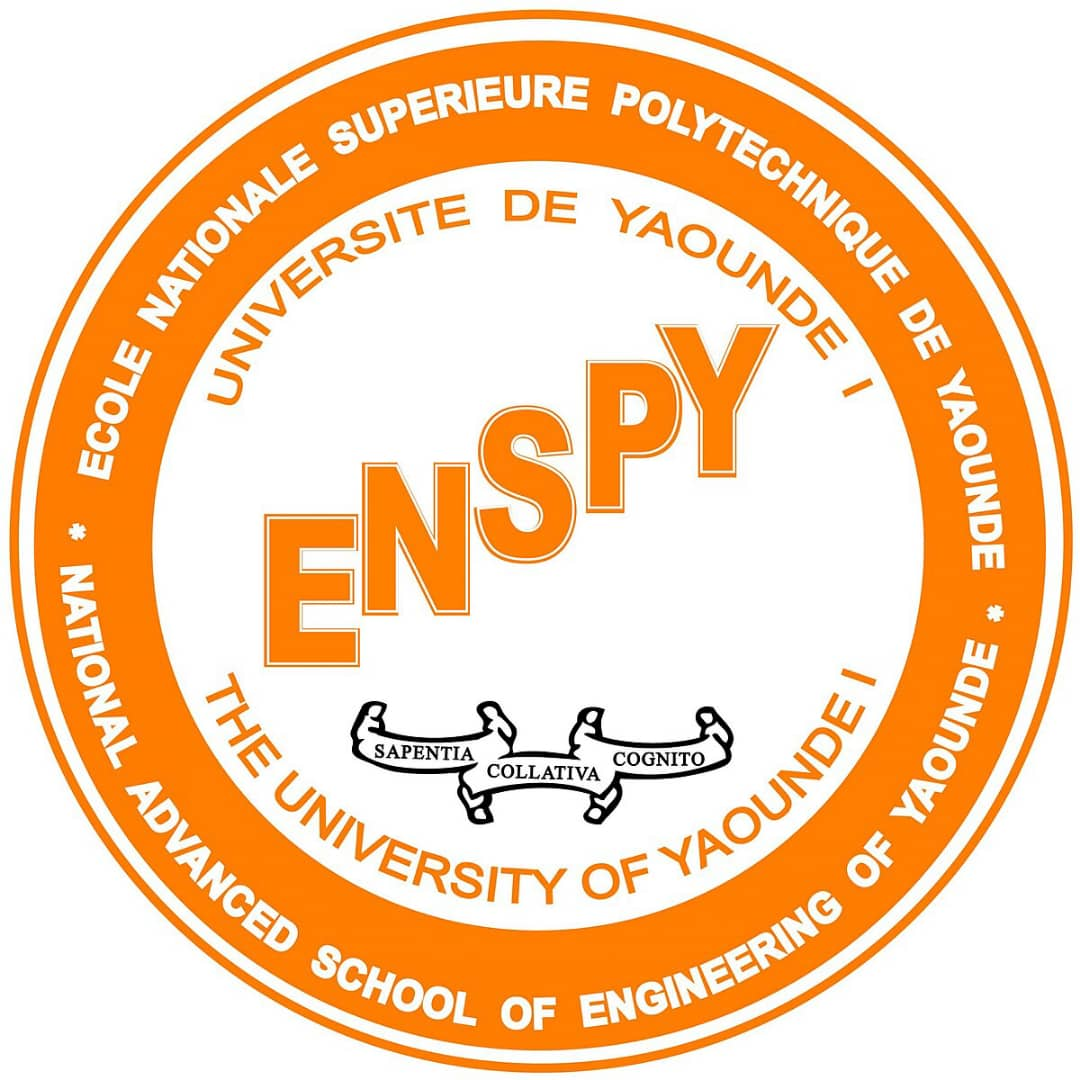
\includegraphics[width=\textwidth, height=3cm]{logo.jpeg}
				\vspace*{\fill} % Espace en bas
			\end{minipage}
			&
			% Colonne de droite (Anglais) - ALIGNÉ EN BAS
			\begin{minipage}[t][5cm][b]{0.36\textwidth}
				\raggedright
				\begin{center}
					{\small \textbf{REPUBLIC OF CAMEROON}}\\
					{\small \textbf{******}}\\
					{\small \textbf{UNIVERSITY OF YAOUNDE I}}\\
					{\small \textbf{******}}\\
					{\small \textbf{NATIONAL ADVANCED SCHOOL OF}}\\
					{\small \textbf{ENGINEERING}}\\
					{\small \textbf{******}}\\
					{\small \textbf{DEPARTMENT OF COMPUTER ENGINEERING}}\\
				\end{center}
			\end{minipage}
		\end{tabular}
		
		\vspace{1.5cm}
		
		% Ligne séparatrice
		\noindent\rule{0.9\textwidth}{0.8pt}\\
		\vspace{0.5cm}
		
		% Thème
		\vspace{0.8cm}
		{\Large \textbf{RESUME DU COURS}}\\
		\vspace{0.5cm}
		{\Large \textbf{"THEORIES ET PRATIQUES DE L'INVESTIGATIONS NUMERIQUES"}}\\
		\vspace{0.8cm}
		
		
\includegraphics[width=0.5\textwidth]{For.jpeg}
		% Ligne séparatrice
		\noindent\rule{0.9\textwidth}{0.8pt}\\
		\vspace{1.5cm}
		
		% Informations étudiant
		\begin{tabular}{@{}>{\bfseries}l l@{}}
			\vspace{0.5cm}
			Réalisé par : & \textbf{NANTIA ZAGUE AXEL FRISKYL} \\
			\vspace{0.5cm}
			Matricule : & \textbf{22P105} \\
			\vspace{0.5cm}
			Spécialité : & \textbf{Cybersécurité et Investigation Numérique (CIN)} \\
			\vspace{0.5cm}
			UE : & \textbf{Introduction aux techniques de l'Investigations Numériques} \\
			\vspace{0.5cm}
			Sous la supervision de : & \textbf{Mr. MINKA MI NGUIDJOI Thierry Emmanuel} \\
			\vspace{0.5cm}
			Année académique : & \textbf{2025/2026} \\
		\end{tabular}
		
	\end{titlepage}
	
	% Page de garde sans en-tête
	\thispagestyle{empty}
	\newpage
	
	% Début du contenu avec en-tête
	\clearpage
	\setcounter{page}{1}
	
	\vspace{1.5cm}
	
	\begin{center}
		\Large \textbf{Résumé du Manuel de Théorie et Pratiques de l'Investigations Numeriques}
	\end{center}
	
		
	\subsection*{}
	L'investigation numérique se révèle comme une discipline philosophique cruciale, interrogeant les fondements de la vérité, la confiance et la justice dans la société digitale contemporaine. Elle marque une transformation ontologique profonde où l'identité humaine intègre désormais une dimension numérique substantielle, posant un paradoxe fondamental entre transparence nécessaire et intimité préservée. Cette discipline émerge dans un contexte de mutation digitale accélérée, nécessitant une réflexion épistémologique approfondie sur la nature même de la preuve et de la vérité à l'ère numérique.
	
	La preuve numérique évolue radicalement de tangible à immatérielle, devenant soumise à des crises de vérité permanentes dues aux manipulations algorithmiques sophistiquées et à la multiplicité des réalités numériques parallèles. L'introduction récente des protocoles Zero-Knowledge Non-Repudiation (ZK-NR) représente une avancée majeure permettant de concilier efficacement confidentialité renforcée et authenticité vérifiable dans les preuves numériques contemporaines. L'investigateur moderne évolue ainsi vers une figure de philosophe-praticien, constamment confronté à des dilemmes éthiques complexes, notamment la gestion quotidienne du trilemme CRO entre confidentialité absolue, fiabilité technique et opposabilité juridique contraignante.
	
	Dans une perspective historique approfondie, le développement de l'investigation numérique traverse plusieurs phases historiques distinctes, débutant significativement dans les années 1970 avec l'émergence des premiers crimes informatiques primitifs et le développement des premiers outils de forensic expérimentaux. Les années 1980-1990 marquent une période cruciale de professionnalisation accélérée avec des cas emblématiques fondateurs comme l'affaire retentissante des "414s" et celle, médiatisée, de Kevin Mitnick, ainsi que des opérations majeures révélant progressivement la nécessité impérieuse de méthodologies standardisées et reproductibles.
	
	\medskip
	La période charnière 2000-2010 se trouve marquée par une standardisation progressive et l'essor significatif de l'e-discovery, illustrée notamment par les affaires complexes d'Enron et le cas médiatique de Gary McKinnon. La décennie 2010-2020 constitue une révolution technologique avec l'avènement du Big Data massif, du cloud computing ubiquitous, de la blockchain disruptive, et de l'intelligence artificielle transformative qui redéfinissent fondamentalement les méthodologies d'investigation traditionnelles. Depuis 2020, l'ère post-quantique naissante et l'IA avancée marquent un tournant décisif, avec l'apparition d'attaques sophistiquées comme l'incident SolarWinds, nécessitant des innovations continues dans les techniques investigatrices et les collaborations internationales renforcées.
	
	Certaines affaires emblématiques particulièrement significatives ont profondément et durablement influencé l'évolution disciplinaire. L'affaire BTK Killer, résolue grâce à l'analyse méticuleuse des métadonnées, souligne définitivement l'importance cruciale des traces numériques infimes. Stuxnet inaugure véritablement l'ère des cyber-armes industrielles sophistiquées et ouvre la voie pionnière à des techniques avancées de reverse engineering complexe et de sandboxing élaboré. L'attaque virale WannaCry illustre parfaitement la propagation rapide et massive de malwares à grande échelle et démontre l'importance critique de la découverte en temps réel des méthodes de génération de domaines évolutives.
	
	\medskip
	D'une part, les chapitres fondamentaux abordent systématiquement les fondements théoriques essentiels, mettant particulièrement en avant l'importance primordiale des traces primaires directes et secondaires indirectes, ainsi que l'application rigoureuse de modèles internationalement reconnus, tels que le modèle DFRWS complet et les normes ISO/IEC contraignantes. Ces fondements solides intègrent nécessairement des notions mathématiques avancées comme l'entropie de Shannon complexe et la théorie des graphes relationnels, qui permettent de mieux comprendre structurellement et analyser efficacement les données numériques massives pour révéler des patterns cachés significatifs, anomalies suspectes ou relations pertinentes essentielles à l'enquête approfondie.
	
	D'autre part, les approches normatives contraignantes et méthodologiques structurées représentent un socle critique indispensable pour la réglementation encadrante et la standardisation impérative des investigations numériques modernes. Les cadres de référence comme ISO/IEC 27037 exhaustif et les directives NIST détaillées fournissent des principes directeurs éprouvés pour la collecte préservante, la préservation intacte et l'analyse rigoureuse des preuves numériques délicates, auxquels s'adjoignent utilement des guides spécifiques spécialisés comme celui de l'ACPO opérationnel. Ces références autorisées définissent des pratiques reconnues internationalement pour garantir irréfutablement la validité juridique incontestable des éléments techniques ainsi que la traçabilité complète et l'intégrité absolue, devenue essentielle dans un contexte juridique de plus en plus complexe et exigeant.
	
	\medskip
	Tout d'abord, la problématique fondamentale du trilemme CRO insoluble met en lumière évidente l'incompatibilité intrinsèque profonde entre trois exigences majeures contradictoires : la confidentialité absolue, la fiabilité technique, et l'opposabilité juridique contraignante. Cette incompatibilité conceptuelle signifie fondamentalement qu'il devient théoriquement impossible d'optimiser simultanément ces trois axes divergents sans faire de compromis inévitables. Pour formaliser mathématiquement cette réalité, des indices quantitatifs précis sont attribués méthodiquement à chaque propriété distinctive et utilisés systématiquement pour évaluer objectivement les primitives cryptographiques variées et les protocoles complexes, orientant ainsi rationnellement la conception vers des solutions hybrides équilibrées.
	
	Ensuite, l'analyse méthodique exhaustive des primitives cryptographiques diverses, symétriques traditionnelles, asymétriques modernes, et post-quantiques émergentes, souligne impartialement des forces distinctives et des faiblesses structurelles propres à chaque type de mécanisme particulier. Par exemple concret, l'AES-256 robuste offre une excellente confidentialité renforcée et une fiabilité éprouvée mais montre une faible opposabilité juridique limitée, tandis que les signatures RSA conventionnelles jouissent d'une grande opposabilité reconnue mais demeurent vulnérables structurellement dans un contexte quantique menaçant. Les primitives modernes innovantes comme CRYSTALS-Kyber prometteur et Dilithium résistant émergent progressivement comme indispensables pour la résistance quantique future, bien que leur maturité juridique complète reste encore à consolider progressivement.
	
	De plus, l'impact majeur croissant de l'informatique quantique révolutionnaire transforme profondément et durablement la conception traditionnelle et l'approche conventionnelle de la forensic numérique classique. Les algorithmes quantiques spécialisés, en particulier ceux de Shor disruptif et Grover performant, remettent radicalement en cause la sécurité supposée des primitives classiques établies, posant la problématique cruciale du \textit{Harvest Now, Decrypt Later} inquiétant, où les données chiffrées aujourd'hui potentiellement peuvent être décryptées demain par des ordinateurs quantiques puissants. Cette menace imminente nécessite une adaptation urgente et une migration accélérée vers des solutions cryptographiques post-quantiques résistantes.
	
	\medskip
	L'équipement technique spécialisé et l'arsenal méthodologique sophistiqué de l'investigation numérique moderne incluent nécessairement une panoplie complète d'outils d'acquisition préservante, d'analyse approfondie et de détection avancée performants, intégrant intelligemment des procédures anti-anti-forensique contre-mesures. L'usage croissant exponentiel de l'intelligence artificielle prédictive permet désormais d'automatiser efficacement la classification automatique des malwares variés, la détection proactive d'anomalies comportementales subtiles, et l'analyse prédictive anticipatrice des menaces émergentes.
	
	Des scripts dédiés personnalisés facilitent opérationnellement l'acquisition sécurisée renforcée de données sensibles avec validation d'intégrité cryptographique, tandis que des plugins spécifiques spécialisés, tels que ceux développés spécifiquement pour Volatility 3 avancé, renforcent significativement l'analyse mémoire complète dans un cadre post-quantique exigeant. Ces avancées techniques remarquables s'accompagnent simultanément d'un enjeu éthique important et juridique fort, où les techniques de préservation cryptographique innovantes (notamment ZK-NR révolutionnaire) assurent simultanément la traçabilité complète et l'opposabilité juridique des preuves digitales, tout en protégeant efficacement la confidentialité légitime des personnes impliquées.
	
	L'évaluation formelle rigoureuse et la cryptanalyse approfondie des protocoles cryptographiques complexes, avec un focus particulier accentué sur le protocole ZK-NR innovant, dévoile une complexité maîtrisée grâce à une conception modulaire flexible et une défense en profondeur stratifiée. Cette architecture résiliente garantit structurellement que la défaillance potentielle d'une couche isolée ne compromet pas la totalité du système intégré, assurant ainsi une robustesse pratique opérationnelle face aux attaques sophistiquées.
	
	\medskip
	Pour illustrer concrètement et pédagogiquement ces concepts abstraits, une vignette pratique réaliste présente une attaque ransomware sophistiquée sur CyberFinance Cameroun survenant en 2025. Cette fintech majeure régionale, avec un portefeuille substantiel d'un demi-million de clients confiants, subit dramatiquement un chiffrement complet malveillant de sa base clients critique et une exfiltration massive illicite de données sensibles, suivie immédiatement d'une demande de rançon exorbitante en Bitcoin anonyme. L'architecture réseau compromise étendue comprend divers éléments vulnérables : serveurs web exposés, bases de données sensibles, API interconnectées, et réseaux internes permeables.
	
	L'alerte opérationnelle est donnée initialement suite à des anomalies réseau détectées subtilement puis confirmée par des alertes IDS corrélées. La réponse immédiate coordonnée a permis d'isoler rapidement le réseau contaminé, de préserver précieusement les données volatiles essentielles, et d'activer efficacement un plan de crise préétabli. L'analyse technique approfondie révèle ultérieurement un ransomware sophistiqué de la famille LockBit notoire, combinant astucieusement chiffrement ChaCha20 rapide et RSA-2048 robuste, avec mécanisme de persistance insidieux via tâche planifiée cachée et compromission complète du MBR système.
	
	L'évaluation objective selon le Trilemme CRO exigeant note des atteintes majeures préoccupantes à la confidentialité des données et à la fiabilité systémique, et constate une faible opposabilité juridique des preuves techniques altérées. Il est recommandé stratégiquement un déploiement immédiat des preuves ZK-NR innovantes, une architecture Q2CSI résiliente, et une migration accélérée vers des signatures post-quantiques durables. La collecte méticuleuse de preuves suit scrupuleusement la norme ISO 27037 contraignante, incluant une acquisition forensique d'image disque validée cryptographiquement par hash sécurisé, avec intégration transparente du protocole ZK-NR avancé pour garantir définitivement l'admissibilité juridique incontestable.
	
	\medskip
	L'analyse approfondie méticuleuse reconstitue minutieusement une chronologie détaillée d'événements critiques successifs, partant de la réception initiale d'un courriel de phishing ciblé jusqu'au déploiement final complet du ransomware destructeur. L'attribution technique précise de l'attaque complexe par analyse détaillée des TTPs MITRE spécifiques indique fortement un groupe affilié LockBit "GoldManager" expérimenté, probablement originaire géographiquement d'Europe de l'Est. Trois serveurs C2 Tor furtifs ont été identifiés positivement, avec une exfiltration data fragmentée sophistiquée de 850 Go volumineux en HTTPS encrypté.
	
	Le plan de remédiation complet propose des actions immédiates prioritaires d'isolation réseau stricte, de réinitialisation complète des accès compromis, de déploiement urgent de solutions EDR avancées et de segmentation réseau renforcée, suivi méthodiquement d'analyses forensiques poussées exhaustives, de reconstruction complète des systèmes affectés, et de renforcement durable par architecture zéro confiance stricte, SOC continu monitoré et migration PQC progressive. La procédure légale camerounaise applicable encadre rigoureusement la gouvernance formelle de l'affaire complexe depuis le dépôt de plainte initial jusqu'au procès potentiel, avec la préparation minutieuse d'un dossier probant réunissant preuves techniques irréfutables, témoignages corroborants, et documentation juridique complète, intégrant légalement les attestations ZK-NR innovantes.
	
	\medskip
	Les cadres légaux internationaux contraignants et régionaux diversifiés forment ensemble l'infrastructure réglementaire essentielle sur laquelle repose solidement l'investigation numérique contemporaine globale. Les législations américaines complexes, européennes unifiées, et africaines émergentes définissent précisément des règles précises contraignantes sur l'authentification formelle des preuves numériques, la protection renforcée des données personnelles sensibles, et les procédures d'enquête encadrées. Les conventions internationales importantes comme la Convention de Budapest fondamentale orientent utilement la coopération transnationale et harmonisent progressivement les pratiques investigatrices au-delà des frontières nationales.
	
	Ces cadres réglementaires diversifiés sont cependant structurellement confrontés à la tension permanente entre exigences contradictoires de transparence démocratique, respect fondamental de la vie privée individuelle, et rapidité opérationnelle des investigations urgentes dans un environnement numérique en perpétuelle évolution rapide. En Afrique particulièrement, les normes nationales disparates et régionales émergentes progressent laborieusement vers une meilleure intégration fonctionnelle, mais restent encore à consolider significativement en termes critiques de formation spécialisée, de délais procéduraux, et de ressources techniques suffisantes.
	
	\medskip
	L'organisation pratique opérationnelle des opérations d'investigation numérique exigeante demande un environnement technique adapté et humain compétent, conforme aux standards internationaux exigeants. La mise en place indispensable de laboratoires spécialisés équipés, intégrant des infrastructures matérielles robustes et logicielles avancées, est absolument primordiale pour garantir des résultats fiables. Des procédures opérationnelles standardisées exhaustives, incluant des checklists détaillées, modèles de rapports standardisés, et scripts d'automatisation efficaces, permettent d'optimiser significativement la fiabilité technique et la reproductibilité scientifique des investigations complexes.
	
	La gestion rigoureuse méticuleuse des chaînes de custody continues garantit juridiquement l'intégrité probante des preuves délicates tout au long du processus legal complet. Enfin, la formation continue obligatoire, la veille technologique permanente, et la participation active à des exercices pratiques réalistes tels que les red teams simulées contribuent ensemble à maintenir un haut niveau d'expertise technique et à anticiper proactivement les évolutions constantes des menaces sophistiquées et des technologies émergentes.
	
	\medskip
	L'analyse post-mortem exhaustive du cas CyberFinance complexe identifie clairement des causes techniques précises, humaines comportementales et procédurales organisationnelles, avec des recommandations hiérarchisées critiques prioritaires, fortes importantes et moyennes complémentaires pour améliorer durablement la résilience organisationnelle. Un framework de résilience post-quantique prospectif est conçu spécifiquement, agissant simultanément sur la prévention proactive, l'intégrité assurée, la traçabilité complète et la cryptographie avancée tout en optimisant continuellement la gestion équilibrée du Trilemme CRO contraignant.
	
	Les recommandations pratiques incluent la mise en œuvre concrète de solutions de détection avancée comportementale, la formation renforcée du personnel technique, la mise à jour régulière des procédures d'urgence testées, et l'adoption progressive de technologies cryptographiques post-quantiques matures. L'importance cruciale des exercices réguliers de simulation d'incidents réalistes et des audits de sécurité périodiques indépendants est également fortement soulignée pour maintenir un niveau de préparation optimal.
	
	\medskip
	Ce cas concret illustre parfaitement la complexité croissante et les défis contemporains multidimensionnels de la forensique numérique moderne dans un monde interconnecté où la technologie quantique disruptive, la cryptographie post-quantique émergente, et la coopération internationale renforcée sont désormais au cœur des stratégies de défense avancées. L'ère post-quantique naissante ouvre simultanément de nouvelles perspectives prometteuses et des impératifs catégoriques exigeants, faisant de l'investigation numérique un acte essentiel de préservation des libertés fondamentales à travers la documentation fidèle du réel digital.
	
	En définitive synthétique, l'investigation numérique moderne représente un domaine technique en constante évolution rapide, nécessitant une adaptation permanente aux nouvelles technologies disruptives et menaces sophistiquées. La formation continue indispensable, la veille technologique permanente, et la participation active à des exercices pratiques réalistes contribuent collectivement à maintenir un haut niveau d'expertise spécialisée dans ce domaine crucial pour la sécurité numérique nationale. L'approche systémique intégrée combinant technique avancée, droit adapté et éthique responsable reste absolument essentielle pour répondre efficacement aux défis complexes de la société digitale contemporaine globale.
	
\end{document}